\subsection{Sätze des Pythagoras}
\begin{Theorem}
  \begin{minipage}{0.5\textwidth}
    In einem rechtwingkligen Dreieck $\Delta ABC$ gilt:\\
    $$a^2+b^2=c^2$$
  \end{minipage}
  \begin{minipage}{0.5\textwidth}
    \definecolor{qqwuqq}{rgb}{0,0.39215686274509803,0}
    \definecolor{ududff}{rgb}{0.30196078431372547,0.30196078431372547,1}
    \begin{tikzpicture}[line cap=round,line join=round,>=triangle 45,x=1cm,y=1cm,scale=0.4]
    \clip(-13,-3) rectangle (0,4);
    \draw[line width=0.5pt,color=qqwuqq,fill=qqwuqq,fill opacity=0.10000000149011612] (-6.851258827998152,2.8478198196798843) -- (-6.633398787368505,2.627871663644841) -- (-6.413450631333462,2.8457317042744883) -- (-6.631310671963109,3.0656798603095314) -- cycle;
    \draw [line width=0.4pt] (-11.704106007375259,-1.9589560257157905)-- (-6.631310671963109,3.0656798603095314);
    \draw [line width=0.4pt] (-6.631310671963109,3.0656798603095314)-- (-1.6066747859377828,-2.007115475102615);
    \draw [line width=0.4pt] (-11.704106007375259,-1.9589560257157905)-- (-1.6066747859377828,-2.007115475102615);
    \begin{scriptsize}
    \draw [fill=ududff] (-11.704106007375259,-1.9589560257157905) circle (2.5pt);
    \draw[color=ududff] (-12,-1.646543156800932) node {$A$};
    \draw [fill=ududff] (-1.6066747859377828,-2.007115475102615) circle (2.5pt);
    \draw[color=ududff] (-1,-1.6903244744253179) node {$B$};
    \draw [fill=ududff] (-6.631310671963109,3.0656798603095314) circle (2.5pt);
    \draw[color=ududff] (-6.509790378375092,3.4) node {$C$};
    \draw[color=black] (-8.611293624345604,0.5425227244183474) node {$b$};
    \draw[color=black] (-4.831506536106975,0.5425227244183474) node {$a$};
    \draw[color=black] (-6.611946786165325,-1.7) node {$c$};
    \end{scriptsize}
    \end{tikzpicture}
  \end{minipage}
\end{Theorem}
\begin{Beweis}
  Man modelliere die 3 Seiten durch Vektoren, $\vv{a}$, $\vv{b}$ und $\vv{c}$.\\
  Es gilt: $$\vv{a} \cdot \vv{b} &= 0 $$
  $$ a_1 b_1+a_2 b_2 &= 0 $$
  Außerdem:
  \begin{center}
    \begin{align*}
      |\vv{a} + \vv{b}| &= \sqrt{(b_1-a_1)^2+(b_2-a_2)^2}\\
      &= \sqrt{{b_1}^2-2b_1 a_2+{a_1}^2 + {b_2}^2-2b_2 a_2+{a_2}^2}\\
      &= \sqrt{{b_1}^2 + {b_2}^2 + {a_1}^2 + {a_2}^2 -2(b_1 a_2 + b_2 a_2)}\\
      &= \sqrt{{b_1}^2 + {b_2}^2 + {a_1}^2 + {a_2}^2}\\
      &= |\vv{c}| \text{, denn $\vv{a} + \vv{b} = \vv{c}$}\\
      \Leftrightarrow |\vv{c}|^2 &= {b_1}^2 + {b_2}^2 + {a_1}^2 + {a_2}^2\\
      \Leftrightarrow |\vv{c}|^2 &= |\vv{a}|^2 + |\vv{b}|^2\\
      \Leftrightarrow c^2 &= a^2 + b^2\\
    \end{align*}
  \end{center}
\end{Beweis}
\begin{Bemerkung}
  Dieser Beweis ist weitaus intuitiver und einfacher, wenn er in der klassischen Geometrie vollführt wird, aber das Ziel ist der Beweis über Vektoren, und somit analytisch.
\end{Bemerkung}
\begin{Theorem}[- Umkehrung]
  \begin{minipage}{0.5\textwidth}
    Falls für ein Dreieck $\Delta ABC$ gilt:\\
    $$a^2+b^2=c^2$$
    Dann ist dieses Dreieck in $C$ rechtwinklig.
  \end{minipage}
  \begin{minipage}{0.5\textwidth}
    \definecolor{qqwuqq}{rgb}{0,0.39215686274509803,0}
    \definecolor{ududff}{rgb}{0.30196078431372547,0.30196078431372547,1}
    \begin{tikzpicture}[line cap=round,line join=round,>=triangle 45,x=1cm,y=1cm,scale=0.4]
    \clip(-13,-3) rectangle (0,4);
    \draw[line width=0.5pt,color=qqwuqq,fill=qqwuqq,fill opacity=0.10000000149011612] (-6.851258827998152,2.8478198196798843) -- (-6.633398787368505,2.627871663644841) -- (-6.413450631333462,2.8457317042744883) -- (-6.631310671963109,3.0656798603095314) -- cycle;
    \draw [line width=0.4pt] (-11.704106007375259,-1.9589560257157905)-- (-6.631310671963109,3.0656798603095314);
    \draw [line width=0.4pt] (-6.631310671963109,3.0656798603095314)-- (-1.6066747859377828,-2.007115475102615);
    \draw [line width=0.4pt] (-11.704106007375259,-1.9589560257157905)-- (-1.6066747859377828,-2.007115475102615);
    \begin{scriptsize}
    \draw [fill=ududff] (-11.704106007375259,-1.9589560257157905) circle (2.5pt);
    \draw[color=ududff] (-12,-1.646543156800932) node {$A$};
    \draw [fill=ududff] (-1.6066747859377828,-2.007115475102615) circle (2.5pt);
    \draw[color=ududff] (-1,-1.6903244744253179) node {$B$};
    \draw [fill=ududff] (-6.631310671963109,3.0656798603095314) circle (2.5pt);
    \draw[color=ududff] (-6.509790378375092,3.4) node {$C$};
    \draw[color=black] (-8.611293624345604,0.5425227244183474) node {$b$};
    \draw[color=black] (-4.831506536106975,0.5425227244183474) node {$a$};
    \draw[color=black] (-6.611946786165325,-1.7) node {$c$};
    \end{scriptsize}
    \end{tikzpicture}
  \end{minipage}
\end{Theorem}
\begin{Beweis}
  Sind Äquivalenzumformungen nicht schön?
\end{Beweis}

\subsection{Euklids Sätze}
\begin{Theorem}[- Kathetensatz]
  \begin{minipage}{0.5\textwidth}
  In einem in $C$ rechtwinkligen Dreieck $\Delta ABC$ mit $h$ der Höhe zu $C$ gilt:\\
    \begin{itemize}
      \item $a^2 = p \cdot c$
      \item $b^2 = q \cdot c$
    \end{itemize}
  \end{minipage}
  \begin{minipage}{0.5\textwidth}
    \definecolor{qqwuqq}{rgb}{0,0.39215686274509803,0}
    \definecolor{ududff}{rgb}{0.30196078431372547,0.30196078431372547,1}
    \begin{tikzpicture}[line cap=round,line join=round,>=triangle 45,x=1cm,y=1cm,scale=.6]
    \clip(-8.311937785825172,-3) rectangle (8.290449729798194,2);
    \draw [shift={(-3.5656013566444793,1.3718053107067734)},line width=0.5pt,color=qqwuqq,fill=qqwuqq,fill opacity=0.16] (0,0) -- (-120.15054216593154:0.48766804060251406) arc (-120.15054216593154:-30.15055075070568:0.48766804060251406) -- cycle;
    \draw [line width=0.4pt] (-5.890547931937073,-2.630796139481519)-- (-3.5656013566444793,1.3718053107067734);
    \draw [line width=0.4pt] (3.459368369267905,-2.708712108658227)-- (-3.5656013566444793,1.3718053107067734);
    \draw [line width=0.4pt] (-5.890547931937073,-2.630796139481519)-- (3.459368369267905,-2.708712108658227);
    \draw [line width=0.4pt] (-3.5656013566444793,1.3718053107067734)-- (-3.5991154959818794,-2.6498914097811452);
    \draw [line width=0.4pt] (-5.890547931937073,-2.630796139481519)-- (-3.5991154959818794,-2.6498914097811452);
    \draw [line width=0.4pt] (3.459368369267905,-2.708712108658227)-- (-3.5991154959818794,-2.6498914097811452);
    \begin{scriptsize}
    \draw [fill=ududff] (-5.890547931937073,-2.630796139481519) circle (2.5pt);
    \draw[color=ududff] (-6.1,-2.3936022538574075) node {$A$};
    \draw [fill=ududff] (3.459368369267905,-2.708712108658227) circle (2.5pt);
    \draw[color=ududff] (3.543814134600391,-2.43) node {$B$};
    \draw [fill=ududff] (-3.5656013566444793,1.3718053107067734) circle (2.5pt);
    \draw[color=ududff] (-3.4786056500758114,1.8) node {$C$};
    \draw[color=black] (-4.9,-0.583811969844107) node {$b$};
    \draw[color=black] (0.07595251253806888,-0.38874475360315236) node {$a$};
    \draw[color=black] (-1.8638825823030425,-2.9) node {$c$};
    \draw[color=black] (-3.75,-0.5079524968615136) node {$h$};
    \draw[color=black] (-4.605660677246067,-2.328579848443756) node {$q$};
    \draw[color=black] (-0.03241816315137868,-2.3719281187195236) node {$p$};
    \end{scriptsize}
    \end{tikzpicture}
  \end{minipage}
\end{Theorem}
\begin{Beweis}
  \begin{itemize}
    \item \begin{align*}
      a^2 &= c^2-b^2 \text{\qquad\qquad $|$Pythagoras}\\
      &= c^2 -(q^2+h^2)\\
      &= c^2 - ((c-p)^2+(a^2-p^2))\\
      &= c^2 - c^2+ 2cp -p^2 - a^2 + p^2\\
      \Leftrightarrow 2a^2&=2cp \\
      \Leftrightarrow a^2&=cp
    \end{align*}
    \item \begin{align*}
      b^2 &= c^2-a^2 \text{\qquad\qquad $|$Pythagoras}\\
      &= c^2 -(p^2+h^2)\\
      &= c^2 - ((c-q)^2+(b^2-q^2))\\
      &= c^2 - c^2+ 2cq -q^2 - b^2 + q^2\\
      \Leftrightarrow 2b^2&=2cq \\
      \Leftrightarrow b^2&=cq
    \end{align*}
  \end{itemize}
\end{Beweis}
\begin{Theorem}[- Höhensatz]
  \begin{minipage}{0.5\textwidth}
    In einem in $C$ rechtwinkligen Dreieck $\Delta ABC$ mit $h$ der Höhe zu $C$ gilt:
    $$h^2=p\cdot q$$
  \end{minipage}
  \begin{minipage}{0.5\textwidth}
    \definecolor{qqwuqq}{rgb}{0,0.39215686274509803,0}
    \definecolor{ududff}{rgb}{0.30196078431372547,0.30196078431372547,1}
    \begin{tikzpicture}[line cap=round,line join=round,>=triangle 45,x=1cm,y=1cm,scale=.6]
    \clip(-8.311937785825172,-3) rectangle (8.290449729798194,2);
    \draw [shift={(-3.5656013566444793,1.3718053107067734)},line width=0.5pt,color=qqwuqq,fill=qqwuqq,fill opacity=0.16] (0,0) -- (-120.15054216593154:0.48766804060251406) arc (-120.15054216593154:-30.15055075070568:0.48766804060251406) -- cycle;
    \draw [line width=0.4pt] (-5.890547931937073,-2.630796139481519)-- (-3.5656013566444793,1.3718053107067734);
    \draw [line width=0.4pt] (3.459368369267905,-2.708712108658227)-- (-3.5656013566444793,1.3718053107067734);
    \draw [line width=0.4pt] (-5.890547931937073,-2.630796139481519)-- (3.459368369267905,-2.708712108658227);
    \draw [line width=0.4pt] (-3.5656013566444793,1.3718053107067734)-- (-3.5991154959818794,-2.6498914097811452);
    \draw [line width=0.4pt] (-5.890547931937073,-2.630796139481519)-- (-3.5991154959818794,-2.6498914097811452);
    \draw [line width=0.4pt] (3.459368369267905,-2.708712108658227)-- (-3.5991154959818794,-2.6498914097811452);
    \begin{scriptsize}
    \draw [fill=ududff] (-5.890547931937073,-2.630796139481519) circle (2.5pt);
    \draw[color=ududff] (-6.1,-2.3936022538574075) node {$A$};
    \draw [fill=ududff] (3.459368369267905,-2.708712108658227) circle (2.5pt);
    \draw[color=ududff] (3.543814134600391,-2.43) node {$B$};
    \draw [fill=ududff] (-3.5656013566444793,1.3718053107067734) circle (2.5pt);
    \draw[color=ududff] (-3.4786056500758114,1.8) node {$C$};
    \draw[color=black] (-4.9,-0.583811969844107) node {$b$};
    \draw[color=black] (0.07595251253806888,-0.38874475360315236) node {$a$};
    \draw[color=black] (-1.8638825823030425,-2.9) node {$c$};
    \draw[color=black] (-3.75,-0.5079524968615136) node {$h$};
    \draw[color=black] (-4.605660677246067,-2.328579848443756) node {$q$};
    \draw[color=black] (-0.03241816315137868,-2.3719281187195236) node {$p$};
    \end{scriptsize}
    \end{tikzpicture}
  \end{minipage}
\end{Theorem}
\begin{Beweis}
  Der ist einfach:
  \begin{align*}
    a^2+b^2 &=c^2\\
    \Leftrightarrow p^2+h^2+q^2+h^2 &= (p+q)^2\\
    \Leftrightarrow p^2+h^2+q^2+h^2 &= p^2+2pq+q^2\\
    \Leftrightarrow h^2+h^2 &= 2pq\\
    \Leftrightarrow 2h^2 &= 2pq\\
    \Leftrightarrow h^2 &= pq\\
  \end{align*}
\end{Beweis}

\subsection{Strahlensätze}
\definecolor{uuuuuu}{rgb}{0.26666666666666666,0.26666666666666666,0.26666666666666666}
\definecolor{ududff}{rgb}{0.30196078431372547,0.30196078431372547,1}
\begin{Theorem}
  \begin{minipage}{0.5\textwidth}
    Sei ein Dreieck $\Delta ABC$ mit M einem Punkt der Geraden $(AB)$ und N einem Punkt der Geraden $(AC)$. Wenn $(BC)//(MN)$, dann gilt:\\
    $$\dfrac{AM}{AB}=\dfrac{AN}{AC}=\dfrac{MN}{BC}$$
  \end{minipage}
  \begin{minipage}{0.5\textwidth}
    \begin{center}
      \begin{tikzpicture}[line cap=round,line join=round,>=triangle 45,x=1cm,y=1cm,scale=0.2]
      \clip(-15,-3) rectangle (10,20);
      \draw [line width=1pt] (-13.88,18.25)-- (6.89,-2);
      \draw [line width=1pt] (-6.52,-2)-- (3.2960189635404364,18.25132707869476);
      \draw [line width=1pt] (-13.88,18.25)-- (3.2960189635404364,18.25132707869476);
      \draw [line width=1pt] (-6.52,-2)-- (6.89,-2);
      \begin{scriptsize}
      \draw [fill=ududff] (-13.88,18.25) circle (2.5pt);
      \draw[color=ududff] (-13.478989755879722,19.31815120175381) node {$C$};
      \draw [fill=ududff] (3.2960189635404364,18.25132707869476) circle (2.5pt);
      \draw[color=ududff] (3.7115390914138193,19.31815120175381) node {$B$};
      \draw [fill=ududff] (-6.52,-2) circle (2.5pt);
      \draw[color=ududff] (-8,-0.5) node {$M$};
      \draw [fill=ududff] (6.89,-2) circle (2.5pt);
      \draw[color=ududff] (7.286777284725581,-0.957857182233367) node {$N$};
      \draw [fill=uuuuuu] (-2.2164992168880455,6.878507902839813) circle (2pt);
      \draw[color=uuuuuu] (-0.8432164151340418,7.31906411461164) node {$A$};
      \end{scriptsize}
      \end{tikzpicture}
    \end{center}
  \end{minipage}
\end{Theorem}
\begin{Beweis}
  test
\end{Beweis}

\begin{Theorem}[- Umkehrung]
  \begin{minipage}{0.5\textwidth}
  Sei ein Dreieck $\Delta ABC$ mit M einem Punkt der Geraden $(AB)$ und N einem Punkt der Geraden $(AC)$. Wenn gilt:\\
  $$\dfrac{AB}{AC}=\dfrac{AM}{AN}$$
    Dann ist $(BC)//(MN)$.
  \end{minipage}
  \begin{minipage}{0.5\textwidth}
    \begin{center}
      \begin{tikzpicture}[line cap=round,line join=round,>=triangle 45,x=1cm,y=1cm,scale=0.2]
      \clip(-15,-3) rectangle (10,20);
      \draw [line width=1pt] (-13.88,18.25)-- (6.89,-2);
      \draw [line width=1pt] (-6.52,-2)-- (3.2960189635404364,18.25132707869476);
      \draw [line width=1pt] (-13.88,18.25)-- (3.2960189635404364,18.25132707869476);
      \draw [line width=1pt] (-6.52,-2)-- (6.89,-2);
      \begin{scriptsize}
      \draw [fill=ududff] (-13.88,18.25) circle (2.5pt);
      \draw[color=ududff] (-13.478989755879722,19.31815120175381) node {$C$};
      \draw [fill=ududff] (3.2960189635404364,18.25132707869476) circle (2.5pt);
      \draw[color=ududff] (3.7115390914138193,19.31815120175381) node {$B$};
      \draw [fill=ududff] (-6.52,-2) circle (2.5pt);
      \draw[color=ududff] (-8,-0.5) node {$M$};
      \draw [fill=ududff] (6.89,-2) circle (2.5pt);
      \draw[color=ududff] (7.286777284725581,-0.957857182233367) node {$N$};
      \draw [fill=uuuuuu] (-2.2164992168880455,6.878507902839813) circle (2pt);
      \draw[color=uuuuuu] (-0.8432164151340418,7.31906411461164) node {$A$};
      \end{scriptsize}
      \end{tikzpicture}
    \end{center}
  \end{minipage}
\end{Theorem}
\begin{Beweis}
  test
\end{Beweis}

\subsection{Der Satz des Apollinius}
\begin{Theorem}
  \begin{minipage}[t]{0.5\textwidth}
    Gegeben sind: Eine Strecke $[AB]$ und eine positive Zahl $\lambda \in \R^{+} \backslash \{1\}$. Dann ist die Punktmenge $$M_{A}=\left\{ X \left| \dfrac{\overline{AX}} {\overline{BX}}=\lambda \right\}$$ ein Kreis, den man \textbf{Kreis des Apollinius} nennt.
  \end{minipage}
  \begin{minipage}[t]{0.5\textwidth}
    \center{Anschaulich:}\\
    \definecolor{xdxdff}{rgb}{0.49019607843137253,0.49019607843137253,1}
    \begin{tikzpicture}[line cap=round,line join=round,>=triangle 45,x=1cm,y=1cm,scale=0.4]
      \clip(-14,-6.5) rectangle (4,3);
      \draw [line width=0.6pt] (-3.467268565272,-2.1740714480434544) circle (4.233988972549521cm);
      \draw [line width=0.6pt] (-6.695919714230329,0.5649930597768731)-- (-5.612633124394338,-2.1755042586210407);
      \draw [line width=0.6pt] (-6.695919714230329,0.5649930597768731)-- (-13.088243523450211,-2.180496945578665);
      \draw [line width=0.6pt] (-13.088243523450211,-2.180496945578665)-- (0.766719463010253,-2.171243722188424);
      \begin{scriptsize}
      \draw [fill=xdxdff] (-6.695919714230329,0.5649930597768731) circle (2pt);
      \draw[color=xdxdff] (-6.4308742689257725,1.3147960193295674) node {$X$};
      \draw [fill=xdxdff] (0.766719463010253,-2.171243722188424) circle (2pt);
      \draw[color=xdxdff] (1.137249163879541,-1.3442743759804054) node {$T_a$};
      \draw [fill=xdxdff] (-5.612633124394338,-2.1755042586210407) circle (2pt);
      \draw[color=xdxdff] (-5.339973593926808,-1.4465463142615582) node {$B$};
      \draw [fill=xdxdff] (-13.088243523450211,-2.180496945578665) circle (2pt);
      \draw[color=xdxdff] (-12.805825088450968,-1.4465463142615582) node {$A$};
      \draw [fill=xdxdff] (-7.701256593554253,-2.1768991738984846) circle (2pt);
      \draw[color=xdxdff] (-7,-1.4124556681678406) node {$T_i$};
      \end{scriptsize}
    \end{tikzpicture}
  \end{minipage}
\end{Theorem}
\begin{\small}
\begin{Beweis}
\begin{enumerate}
  \item {Die Ausgangspunkte:  \vartriangleright $A(0|0)$ \qquad \vartriangleright $B(b|0)$ \qquad \vartriangleright $T_{i}(t_{i}|0)$ \qquad \vartriangleright $T_{a}(t_{a}|0)$ \qquad \vartriangleright $X(x|y)$
  }

  \item {Nun gilt:\\
  \begin{minipage}[t]{0.5\textwidth}
  \begin{array}{rccl}
  &$\dfrac{\overline{AT_{i}}}{\overline{T_{i}B}}$ & $=$ & $\lambda$\\
  $\Leftrightarrow & \dfrac{t_{i}}{b-t_{i}} $& $= $& $\lambda$\\
  $\Leftrightarrow & $t_{i}$&$=$&$\lambda \cdot b - \lambda \cdot t_{i}$\\
  $\Leftrightarrow & \lambda \cdot t_{i} + t_{i}$ &$=$& \lambda \cdot b$\\
  $\Leftrightarrow & (\lambda + 1)\cdot t_{i}$&$=$& $\lambda \cdot b$\\
  $\Leftrightarrow & t_{i} $&$=$& $ \dfrac {\lambda}{\lambda +1}\cdot b$
  \end{array}
  \end{minipage}
  \begin{minipage}[t]{0.5\textwidth}
  \begin{array}{rccl}
  &$\dfrac{\overline{AT_{a}}}{\overline{T_{a}B}} $&$ = $&$ \lambda$\\
  $\Leftrightarrow $&$ \dfrac{t_{a}}{t_{a}-b} $&$ = $& $\lambda$\\
  $\Leftrightarrow $&$ t_{a}$&$=$&$\lambda \cdot t_{a} - \lambda \cdot b$\\
  $\Leftrightarrow & \lambda \cdot t_{a} - t_{a} $&$=$&$\lambda \cdot b$\\
  $\Leftrightarrow & (\lambda -1 \cdot )t_{a} $&$=$&$\lambda \cdot b$\\
  $\Leftrightarrow & t_{a} $&$=$&$ \dfrac{\lambda}{\lambda -1}\cdot b$\\
  \end{array}
  \end{minipage}\\
  \begin{center}
  \begin{array} {rccccccl}
  $t_{i} + t_{a} $ & $=$ & $\dfrac {\lambda}{\lambda +1}\cdot b + $\dfrac {\lambda}{\lambda -1}\cdot b  $ &$=$& $(\dfrac{\lambda}{\lambda+1} + \dfrac{\lambda}{\lambda-1})\cdot b$ & $=$ & $\dfrac{\lambda^2}{\lambda^2 -1}\cdot 2b$ \qquad \textcolor{red}{(1)}\\
  \end{array}
  \\
  \begin{array} {rcccccl}
  $t_{i} \cdot t_{a} $ & $=$ & $\dfrac {\lambda}{\lambda +1}\cdot b \cdot $\dfrac {\lambda}{\lambda +1}\cdot b $ & $=$ & $\dfrac{\lambda^2}{\lambda^2 -1}\cdot b^2$ \qquad \textcolor{red}{(2)}\\ \\
  \end{array}
  \end{center}
  }

  \item{$T_{i}$ und $T_{a}$ in Abhängigkeit von $b$ und $\lambda$ jetzt auch noch $X$:
  \begin{array}{rccll}
                    &$ \dfrac{\overline{AX}}{\overline{XB}}$        & $=$ & $\lambda$ \\
  $\Leftrightarrow $&$ \dfrac{(\overline{AX})^2}{(\overline{XB})^2}$& $=$ & $\lambda^2$ \\
  $\Leftrightarrow $&$ \dfrac{x^2+y^2}{(x-b)^2+y^2} $               & $=$ & $\lambda^2$ \\
  $\Leftrightarrow $&$ x^2+y^2 $                                    & $=$ & $\lambda^2 \cdtot [(x-b)^2+y^2]$ \\
  $\Leftrightarrow $&$ 0 $                                          & $=$ & $\lambda^2 \cdot (x-b)^2 +\lambda^2 y^2 -x^2 -y^2$\\
                    &                                               & $=$ & $ x^2\cdot \lambda^2 - 2bx\cdot \lambda^2 +b^2\cdot \lambda^2 +y^2\cdot \lambda^2 -x^2-y^2 $ \textcolor{red}{(3)}
  \end{array}
  }

  \item{$\vv{T_{i}X} = \left(\begin{array}{c} x-t_{i} \\ y \end{array}\right); \vv{T_{a}X} = \left(\begin{array}{c} x-t_{a} \\ y \end{array}\right)$
  \begin{center}
  \begin{array}{rccl}
  $\vv{T_{i}X} \cdot \vv{T_{a}X}$ &$=$& $(x-t_{i})\cdot (x-t_{a}) +y^2$\\
  & $=$ & $x^2 -(t_{i} +t_{a})x + t_{i}\cdot t_{a} + y^2$ & $Benutze (1) und (2) \\
  & $=$ & $x^2 - \dfrac{\lambda^2}{\lambda^2 - 1} \cdot 2bx + \dfrac{\lambda^2}{\lambda^2 - 1} \cdot b^2 +y^2$\\
  & $=$ & $\dfrac{x^2 \cdot (\lambda^2 -1) - 2bx\cdot \lambda^2 + b^2\cdot \lambda^2 + y^2 \cdot (\lambda^2 -1)}{\lambda^2 -1}$\\
  & $=$ & $\dfrac{x^2 \cdot \lambda^2 - 2bx\cdot \lambda^2 b^2\cdot \lambda^2 +y^2\cdot \lambda^2 -x^2 -y^2} {\lambda^2 -1}$ &  $Benutze (3) \\
  & $=$ & $0$\\
  \\
  \end{array}
  \end{center}
  }

  $\Rightarrow \vv{T_{i}X} \bot \vv{T_{a}X} \forall X \Rightarrow \vv{T_{i}X},\vv{T_{a}X}\in$ Thaleskreis über $T_{i}$ und $T_{a}$.
  \end{enumerate}
\end{Beweis}
\begin{Bemerkung}
  \begin{minipage}{0.5\textwidth}
    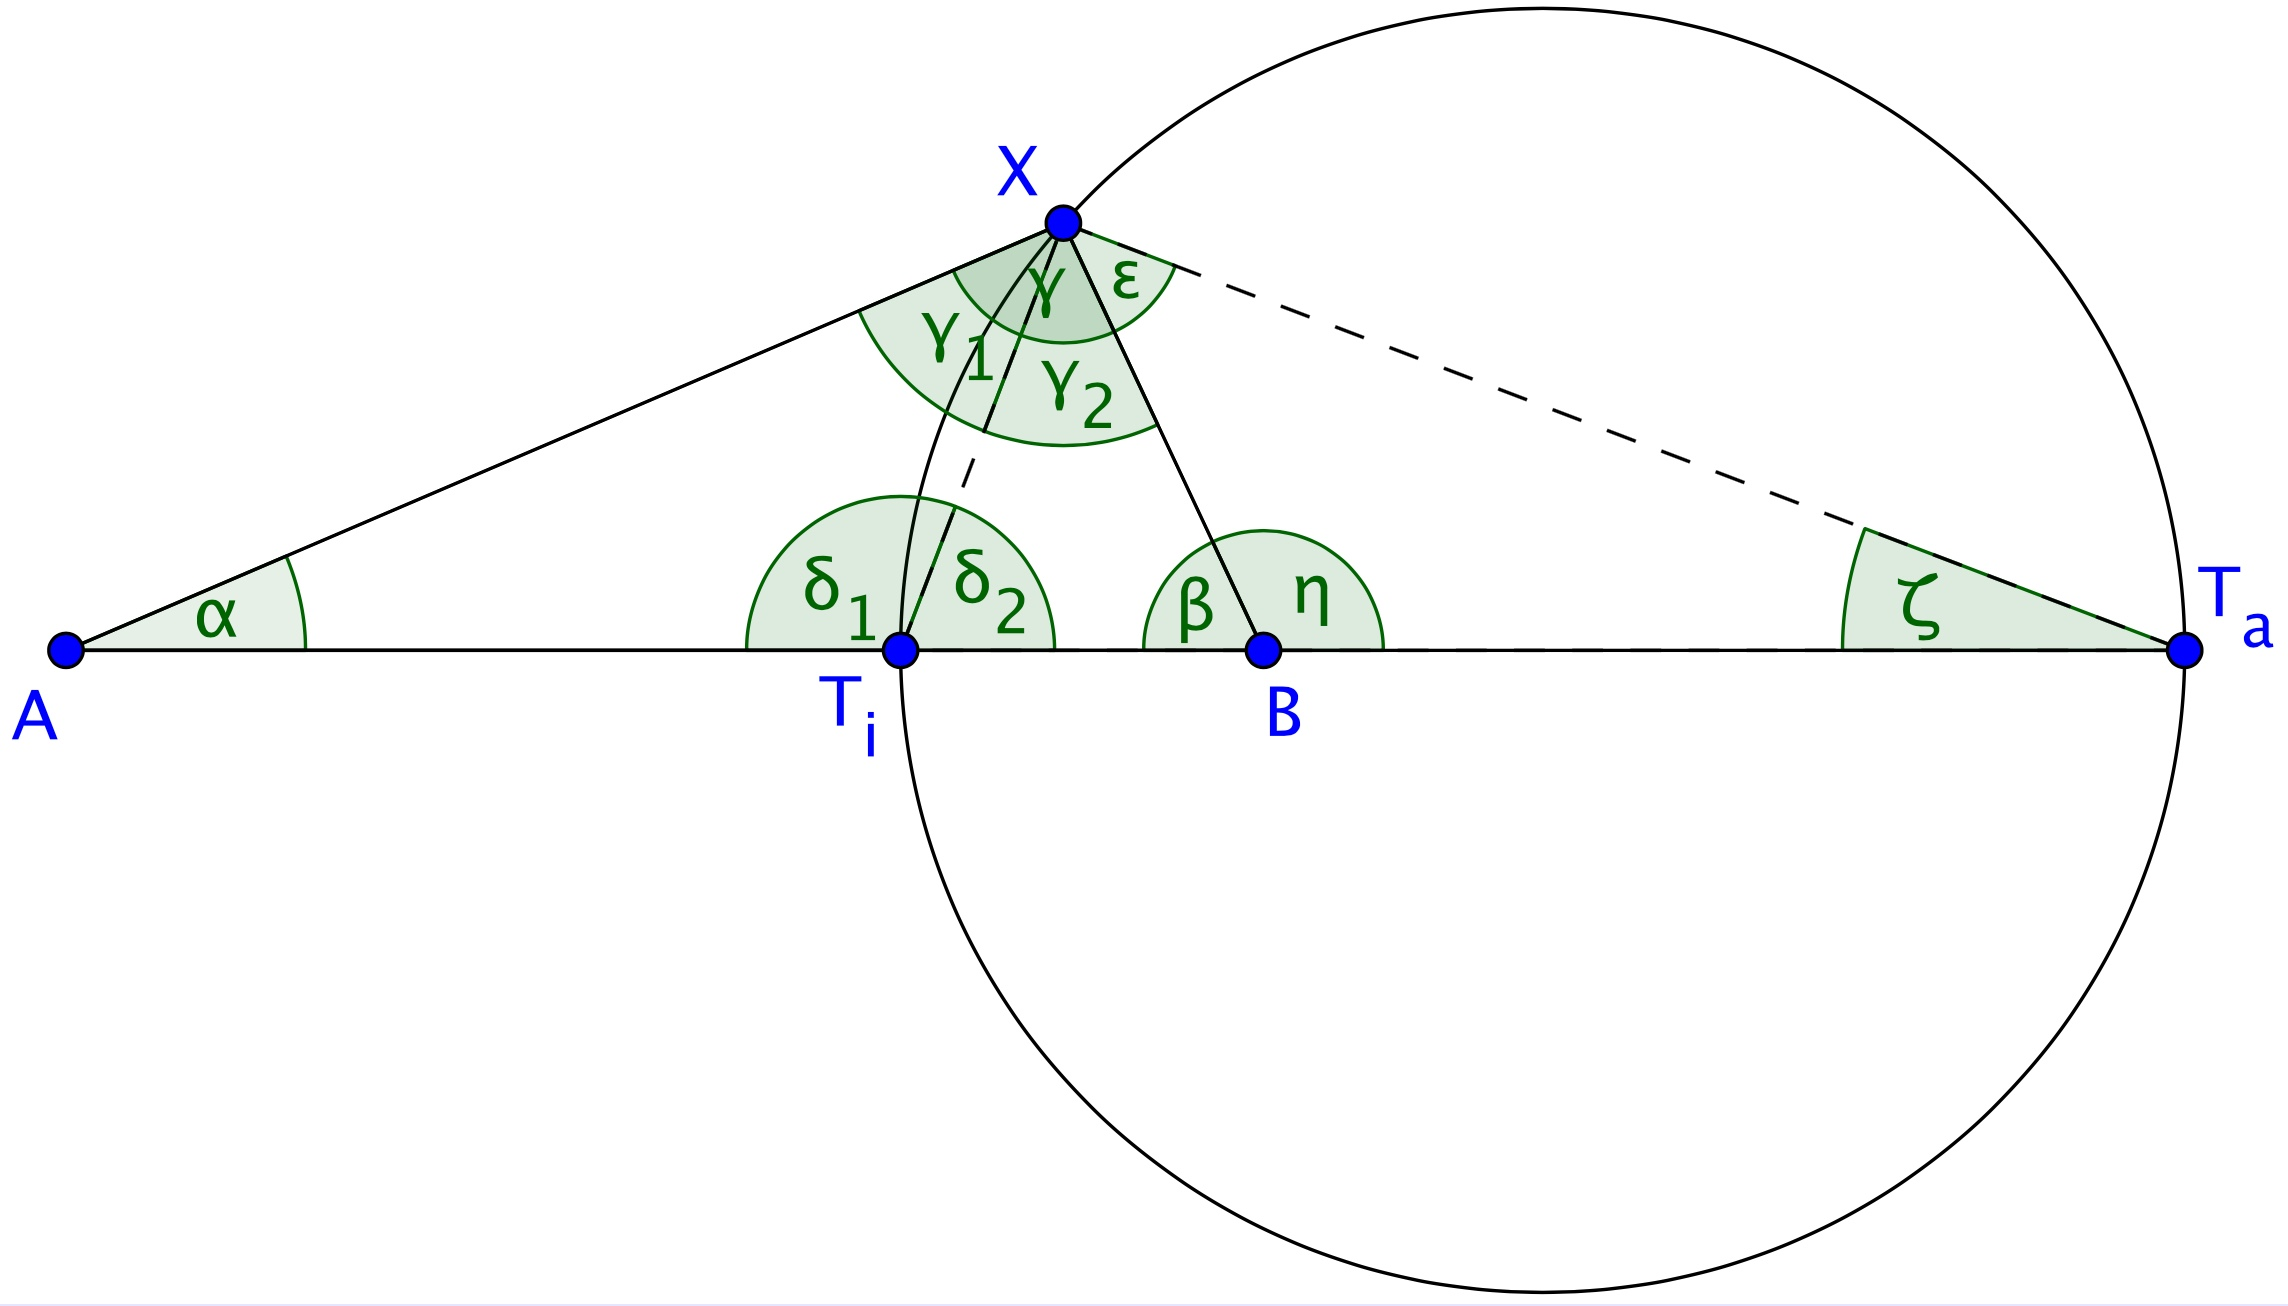
\includegraphics[width=8cm]{kap5/Apollinius_Winkel}
  \end{minipage}
  \begin{minipage}{0.5\textwidth}
    Die Figur und die Zusammenh"ange, die man durch den Satz des Apollinius erhalten hat, kann man benutzen, um ein wenig mit Winkeln zu spielen:
  \end{minipage}\\
  Über diese 10 Winkel lassen sich einige Beziehungen aufstellen:\\
  \begin{array}{rcccl}
  $\vartriangleright \alpha + \beta + \gamma = 180 $ & $\vartriangleright \beta + \gamma_{2} + \delta_{2} = \ang{180} $ & $\vartriangleright \delta_{1} + \delta_{2} = \ang{180} $ & $\vartriangleright \alpha + \gamma + \epsilon + \zeta = \ang{180} $ &$\vartriangleright \epsilon + \zeta + \eta = \ang{180}$\\
  $\vartriangleright \aplha + \gamma_{1} + \delta_{1} = \ang{180} $ & $\vartriangleright \gamma_{1} + \gamma_{2} = \gamma $ & $\vartriangleright \gamma_{2} + \epsilon = \ang{90} $ & $\vartriangleright \beta + \eta = \ang{180} $ &$\vartriangleright \gamma_{2} + \delta_{2} + \epsilon + \zeta = \ang{180}$
  \end{array}
  \\
  Löst man dieses Gleichungssystem, erhält man $\gamma_{1} = \gamma_{2}$, was bedeutet, dass die Gerade $T_{i}X$ Winkelhalbierende des Winkels $\gamma = \angle AXB$ ist:
\end{Bemerkung}
\end{small}
